\chapter{NP-ongelmat}

Olemme tässä kirjassa tutustuneet menetelmiin, joiden avulla voimme
ratkaista tehokkaasti ongelmia.
Kuitenkin on myös monia ongelmia, joiden ratkaisemiseen ei tällä
hetkellä tunneta mitään tehokasta algoritmia.
Jos vastaamme tulee tällainen ongelma, hyvät neuvot ovat kalliit.

Vaikeiden ongelmien yhteydessä vastaan tulee usein
kirjainyhdistelmä NP.
Erityisen tunnettu on P vs. NP -ongelma,
jonka ratkaisijalle on luvattu miljoonan dollarin potti.
Hankalalta tuntuvasta ongelmasta saatetaan mainita, että
se on NP-täydellinen tai NP-vaikea.
Nyt on aika selvittää, mitä nämä käsitteet oikeastaan tarkoittavat.

\section{Luokat P ja NP}

Keskitymme tässä luvussa \emph{päätösongelmiin}, joissa algoritmin tulee
antaa vastaus ''kyllä'' tai ''ei''.
Esimerkiksi ongelma 
''onko verkossa polkua solmusta $a$ solmuun $b$?'' on päätösongelma.
Tulemme huomaamaan, että voimme muotoilla monenlaisia ongelmia
päätösongelmina eikä tämä rajoita juurikaan, mitä ongelmia voimme tarkastella.

\subsubsection{Luokka P}

Luokka P sisältää päätösongelmat, joiden ratkaisemiseen on
olemassa \emph{polynominen} algoritmi eli algoritmi, jonka aikavaativuus
on enintään $O(n^k)$, missä $k$ on vakio.
Lähes kaikki tässä kirjassa esitetyt algoritmit
ovat toimineet polyonmisessa ajassa.
Tuttuja polynomisia aikavaativuuksia ovat esimerkiksi
$O(1)$, $O(\log n)$ $O(n)$, $O(n \log n)$, $O(n^2)$ ja $O(n^3)$.

Esimerkiksi ongelma ''onko verkossa polkua solmusta $a$ solmuun $b$?''
kuuluu luokkaan P, koska voimme ratkaista sen monellakin tavalla
polynomisessa ajassa.
Voimme vaikkapa aloittaa syvyyshaun solmusta $a$ ja tarkastaa,
pääsemmekö solmuun $b$.
Tuloksena on algoritmi, jolla on polynominen aikavaativuus
$O(n+m)$, joten ongelma kuuluu luokkaan P.

Luokan P tarkoituksena on kuvata ongelmia, jotka voimme
ratkaista jossain mielessä \emph{tehokkaasti}.
Tässä tehokkuuden määritelmä on varsin karkea:
pidämme algoritmia tehokkaana, jos sillä on mikä tahansa
polynominen aikavaativuus.
Onko $O(n^{100})$-aikainen algoritmi siis tehokas?
Ei, mutta käytännössä vakio $k$ on yleensä pieni ja
on osoittautunut, että polynominen aikavaativuus 
on toimiva tehokkuuden mittari.


\subsubsection{Luokka NP}

Luokka NP sisältää päätösongelmat, joissa jokaisessa
''kyllä''-tapauksessa on olemassa
\emph{todiste}, jonka avulla voimme
\emph{tarkastaa} polynomisessa ajassa, että vastaus on oikein.
Todiste on merkkijono, jonka koko on polynominen
suhteessa syötteeseen,
ja se antaa meille lisätietoa siitä,
minkä takia ''kyllä''-vastaus pitää paikkansa syötteelle.

Esimerkki luokkaan NP kuuluvasta ongelmasta on
''onko verkossa polkua solmusta $a$ solmuun $b$,
joka kulkee tasan kerran jokaisen verkon solmun kautta?''.
Tämän ongelman ratkaisemiseen ei tunneta tehokasta algoritmia,
mutta jokaisessa ''kyllä''-tapauksessa on olemassa todiste:
halutunlainen polku solmusta $a$ solmuun $b$.
Voimme tarkastaa helposti polynomisessa ajassa,
että todisteen kuvaamalla polulla on vaaditut ominaisuudet.

Jos vastaus syötteeseen on ''ei'', tähän ei tarvitse
liittyä tehokkaasti tarkastettavaa todistetta.
Usein olisikin hankalaa antaa todiste siitä, että jotain
asiaa \emph{ei} ole olemassa.
Äskeisessä esimerkissä meidän oli helppoa todistaa
polun olemassaolo, koska voimme vain näyttää kyseisen polun,
mutta meillä ei ole vastaavaa keinoa todistaa, että polkua ei ole olemassa.

Huomaa, että kaikki luokan P ongelmat kuuluvat myös
luokkaan NP. Tämä johtuu siitä, että luokan P ongelmissa
voimme tarkastaa ''kyllä''-vastauksen
\emph{tyhjän} todisteen avulla: voimme saman tien ratkaista
koko ongelman alusta alkaen polynomisessa ajassa.

\subsubsection{P vs. NP}

Äkkiseltään tuntuu selvältä, että luokassa NP täytyy olla
enemmän ongelmia kuin luokassa P.
Luokassa NP meidän riittää vain pystyä tarkastamaan ''kyllä''-vastauksen
todiste, mikä tuntuu helpommalta kuin muodostaa ongelman ratkaisu tyhjästä.
Monet uskovatkin, että luokka NP on suurempi kuin luokka P --
mutta kukaan ei ole onnistunut todistamaan asiaa.

Tietojenkäsittelytieteen merkittävä avoin ongelma onkin,
päteekö $\textrm{P}=\textrm{NP}$ vai $\textrm{P} \neq \textrm{NP}$.
Monet tutkijat ovat tarttuneet haasteeseen
70-luvulta lähtien, mutta kaikki ovat epäonnistuneet.
Ongelman ratkaisija saisi maineen ja kunnian lisäksi
myös tuntuvan rahallisen korvauksen, koska
Clay-instituutti on luvannut miljoonan dollarin palkinnon
sille, joka todistaa, että $\textrm{P}=\textrm{NP}$ tai $\textrm{P} \neq \textrm{NP}$.
Voi olla kuitenkin, että tämä on yksi \emph{vaikeimmista}
tavoista ansaita miljoona dollaria.

Jos pätee $\textrm{P} \neq \textrm{NP}$, kuten uskotaan,
vaikeutena on keksiä keino todistaa, että jotakin
luokan NP ongelmaa on mahdotonta ratkaista
polynomisessa ajassa.
Tämän todistaminen on vaikeaa, koska meidän pitää näyttää,
että tehokasta algoritmia ei ole olemassa,
vaikka laatisimme algoritmin miten tahansa.
Vaikka moni on koettanut tuloksetta ratkoa
tunnettuja NP-ongelmia, kysymys saattaa silti olla siitä,
että tehokas algoritmi olisi olemassa mutta kukaan ei
vain ole vielä löytänyt sitä.

\section{NP-täydellisyys}

Sanomme, että ongelma on \emph{NP-täydellinen},
jos se kuuluu luokkaan NP ja mikä tahansa luokan NP
ongelma voidaan \emph{palauttaa} siihen polynomisessa ajassa.
NP-täydelliset ongelmat ovat luokan NP vaikeimpia ongelmia:
jos voisimme ratkaista jonkin NP-täydellisen ongelman tehokkaasti,
voisimme ratkaista minkä tahansa luokan NP ongelman tehokkaasti.

Kiinnostava ilmiö on, että lähes kaikki tunnetut luokan NP
ongelmat joko kuuluvat myös luokkaan P tai ovat
NP-täydellisiä.
Nykyään tunnetaankin tuhansia erilaisia NP-täydellisiä ongelmia.
Jos keksisimme mihin tahansa niistä polynomisessa ajassa toimivan
ratkaisun, olisimme samalla onnistuneet todistamaan, että $P=NP$.

\subsection{SAT-ongelma}

Ensimmäinen löydetty NP-täydellinen ongelma oli
SAT-ongelma, jossa annettuna on konjunktiivisessa
normaalimuodossa oleva looginen kaava ja haluamme
selvittää, voimmeko valita muuttujien arvot niin,
että kaava on tosi.
Konjunktiivinen normaalimuoto tarkoittaa,
että kaava koostuu lausekkeista, jotka on yhdistetty
ja-operaatiolla ($\land$), ja jokainen lauseke koostuu
muuttujista ja niiden negaatioista, jotka on yhdistetty
tai-operaatiolla ($\lor$).

Esimerkiksi kaava
\[(\neg x_1 \lor x_3) \land (x_1 \lor x_2 \lor x_3) \land (\neg x_2 \lor \neg x_3)\]
on mahdollista saada todeksi, koska voimme esimerkiksi asettaa
muuttujat $x_1$ ja $x_2$ epätosiksi ja muuttujan $x_3$ todeksi.
Vastaavasti kaava
\[(x_1 \lor x_2) \land (\neg x_1 \lor x_2) \land (x_1 \lor \neg x_2) \land (\neg x_1 \lor \neg x_2) \]
ei ole tosi, vaikka valitsisimme muuttujien arvot miten tahansa.

Kun haluamme osoittaa, että SAT on NP-täydellinen ongelma,
meidän täytyy näyttää, että se kuuluu luokkaan NP ja mikä
tahansa luokan NP ongelma voidaan palauttaa siihen.
Luokkaan NP kuuluminen on helppoa näyttää:
''kyllä''-tapauksessa todiste on jokaiselle muuttujalle valittu arvo.
Huomattavasti vaikeampaa on osoittaa, että \emph{jokainen} luokan
NP ongelma voidaan palauttaa SAT-ongelmaan polynomisessa ajassa.

Tässä kirjassa emme käsittele todistusta yksityiskohtaisesti,
mutta voimme kuitenkin kuvailla sen perusideaa.
Tarkastellaan tiettyä luokan NP ongelmaa,
joka meidän täytyy pystyä palauttamaan SAT-ongelmaan.
Koska ongelma voi olla mikä tahansa luokkaan NP kuuluva, tiedämme siitä vain,
että on olemassa algoritmi, joka tarkastaa
polynomisessa ajassa ''kyllä''-tapauksen todisteen.
Tämä vastaa sitä, että on olemassa epädeterministinen
Turingin kone, joka \emph{arvaa} ensin todisteen sisällön ja
tarkastaa sitten, että todiste on kelvollinen.
Ideana on muodostaa looginen kaava, joka luonnehtii tällaisen
Turing-koneen laskentaa ''kyllä''-tapauksessa:
koneen tulee käsitellä syöte jollakin tavalla,
muodostaa todiste ja tarkastaa se.
Kaavan tarkka sisältö riippuu siitä, miten kone on rakentunut,
mutta voimme aina muodostaa kaavan, kunhan tiedämme koneen rakenteen
ja annetun syötteen.
Tuloksena on looginen kaava, jonka voi saada todeksi tarkalleen silloin,
kun vastaus syötteeseen on ''kyllä'',
joten olemme palauttaneet ongelman SAT-ongelmaan.

\subsection{Ongelmien palautukset}

Nyt kun tiedämme, että SAT-ongelma on NP-täydellinen,
voimme alkaa osoittaa muita ongelmia NP-täydellisiksi palautusten avulla.
Ideana on, että jos ongelma $A$ on NP-täydellinen ja
voimme palauttaa sen polynomisessa ajassa ongelmaksi $B$,
myös ongelma $B$ on NP-täydellinen.

\subsubsection{Palautus SAT $\rightarrow$ 3SAT}

Aloitamme osoittamalla, että 3SAT-ongelma on NP-täydellinen.
3SAT-on\-gelma on SAT-ongelman erikoistapaus, jossa jokaisessa
$\land$-merkeillä yhdistetyssä lausekkeessa on tarkalleen kolme muuttujaa.
Haluamme näyttää, että voimme muuttaa minkä tahansa
SAT-ongelman syötteen 3SAT-ongelman syötteeksi,
jonka totuusarvo on sama.

Ideana on muokata jokaista lauseketta niin, 
että tuloksena on yksi tai useampia kolmen muuttujan lausekkeita.
Merkitään $k$:lla lausekkeen muuttujien määrää.
Jos $k=1$ tai $k=2$, toistamme viimeistä muuttujaa uudestaan,
jotta saamme aikaan kolme muuttujaa.
Esimerkiksi jos lauseke on $(x_1)$, muutamme sen muotoon
$(x_1 \lor x_1 \lor x_1)$, ja jos lauseke on $(x_1 \lor x_2)$, muutamme
sen muotoon $(x_1 \lor x_2 \lor x_2)$.

Jos $k=3$, meidän ei tarvitse tehdä mitään, koska lausekkeessa
on valmiiksi kolme muuttujaa. Jos sitten $k>3$,
jaamme lausekkeen osiin, jotka ketjutetaan apumuuttujien avulla.
Ketjun jokaisessa kohdassa vasemman lausekkeen viimeinen
muuttuja on $a_i$ ja oikean lausekkeen ensimmäinen muuttuja on $\neg a_i$.
Tämä takaa, että ainakin yksi alkuperäinen muuttuja saa oikean arvon.
Esimerkiksi jos lauseke on $(x_1 \lor x_2 \lor x_3 \lor x_4 \lor x_5)$,
muutamme sen kolmeksi lausekkeeksi $(x_1 \lor x_2 \lor a_1)$,
$(\neg a_1 \lor x_3 \lor a_2)$ ja $(\neg a_2 \lor x_4 \lor x_5)$.

Tämä palautus osoittaa, että 3SAT on NP-täydellinen ongelma --
eli saimme tietää, että
SAT-ongelman oleellinen vaikeus syntyy jo silloin, kun lausekkeissa
on vain kolme muuttujaa\footnote{Entä ongelma 2SAT, jossa jokaisessa lausekkeessa
on kaksi muuttujaa? Tämä \emph{ei} ole NP-täydellinen ongelma,
vaan kuuluu luokkaan P.}.
Palautuksen hyötynä on myös se, että kolmen muuttujan lausekkeita
on helpompaa käsitellä myöhemmissä todistuksissa
kuin vaihtelevan pituisia lausekkeita.

\subsubsection{Palautus 3SAT $\rightarrow$ solmupeite}

\begin{figure}
\center
\begin{center}
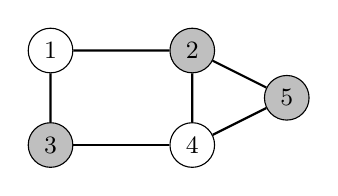
\begin{tikzpicture}[scale=0.6]
\small
\node[draw, circle] (1) at (1,3) {$1$};
\node[draw, circle, fill=lightgray] (2) at (4,3) {$2$};
\node[draw, circle, fill=lightgray] (3) at (1,1) {$3$};
\node[draw, circle] (4) at (4,1) {$4$};
\node[draw, circle, fill=lightgray] (5) at (6,2) {$5$};

\path[draw,thick,-] (1) -- (2);
\path[draw,thick,-] (1) -- (3);
\path[draw,thick,-] (3) -- (4);
\path[draw,thick,-] (2) -- (4);
\path[draw,thick,-] (2) -- (5);
\path[draw,thick,-] (4) -- (5);
\end{tikzpicture}
\end{center}
\caption{Solmut $\{2,3,5\}$ muodostavat solmupeitteen.}
\label{fig:solpei}
\end{figure}

Seuraavaksi osoitamme, että on NP-täydellinen ongelma tarkastaa,
onko verkossa \emph{solmupeitettä}, jossa on enintään $k$ solmua.
Solmupeite on verkon solmujen osajoukko, joka on valittu niin,
että jokaisessa kaaressa ainakin toinen päätesolmu kuuluu
solmupeitteeseen.
Esimerkiksi kuvassa \ref{fig:solpei} on verkko ja sen solmupeite,
johon kuuluu kolme solmua.

Kun haluamme palauttaa 3SAT-ongelman solmupeiteongelmaan,
meidän täytyy näyttää, että voimme tulkita minkä tahansa
3SAT-ongelman tapauksen verkon solmupeitteen etsimisenä.
Meidän tulee siis pystyä muuttamaan looginen kaava verkoksi,
jonka jokin solmupeite vastaa sitä, että kaava on totta.
Tarkastelemme esimerkkinä kaavaa
\[(x_1 \lor \neg x_2 \lor x_3) \land (\neg x_1 \lor \neg x_3 \lor x_4).\]

Oletamme, että kaavassa esiintyy $n$ muuttujaa $x_1,x_2,\dots,x_n$
ja siinä on $m$ lauseketta.
Muodostamme verkon, jossa on ensinnäkin $n$ paria solmuja,
jotka vastaavat muuttujia ja niiden negaatioita.
Jokaisen solmun $x_i$ ja $\neg x_i$ välillä on kaari.
Lisäksi verkossa on $m$ kolmen solmun ryhmää,
jotka vastaavat lausekkeita.
Kussakin ryhmässä kaikki solmut ovat yhteydessä toisiinsa,
minkä lisäksi kukin solmu on yhteydessä sitä vastaavaan solmuun pareissa.
Verkossa on siis $2n+3m$ solmua ja $n+6m$ kaarta.
Kuva \ref{fig:solko1} näyttää esimerkkikaavaamme vastaavan verkon.

\begin{figure}
\center
\begin{center}
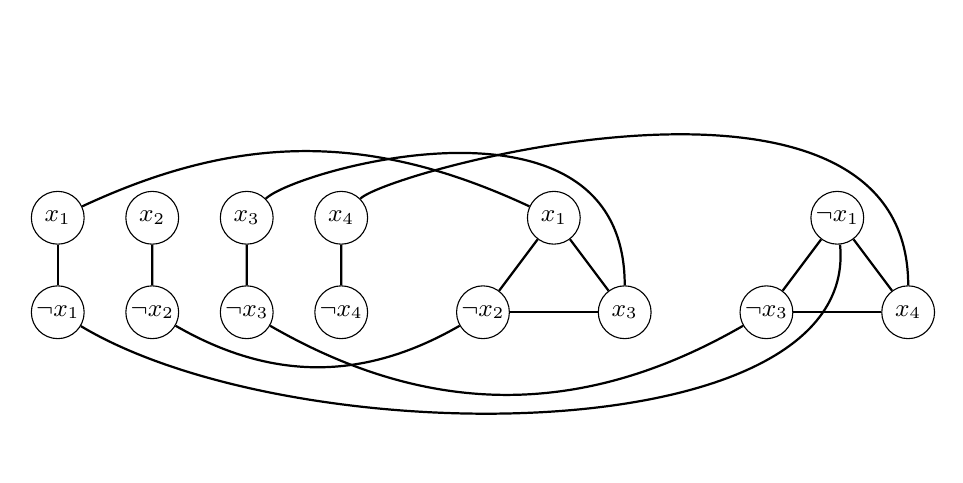
\begin{tikzpicture}[scale=0.6]
\small
\node[draw, circle] (a1) at (0,0) {$x_1$};
\node[draw, circle] (a2) at (2,0) {$x_2$};
\node[draw, circle] (a3) at (4,0) {$x_3$};
\node[draw, circle] (a4) at (6,0) {$x_4$};
\node[draw, circle] (b1) at (0,-2) {\phantom{$x_1$}};
\node[draw, circle] (b2) at (2,-2) {\phantom{$x_2$}};
\node[draw, circle] (b3) at (4,-2) {\phantom{$x_3$}};
\node[draw, circle] (b4) at (6,-2) {\phantom{$x_4$}};
\node at (0,-2) {$\neg x_1$};
\node at (2,-2) {$\neg x_2$};
\node at (4,-2) {$\neg x_3$};
\node at (6,-2) {$\neg x_4$};

\node[draw, circle] (c1) at (10.5,0) {$x_1$};
\node[draw, circle] (c2) at (9,-2) {\phantom{$x_2$}};
\node[draw, circle] (c3) at (12,-2) {$x_3$};
\node at (9,-2) {$\neg x_2$};

\node[draw, circle] (d1) at (16.5,0) {\phantom{$x_1$}};
\node[draw, circle] (d2) at (15,-2) {\phantom{$x_3$}};
\node[draw, circle] (d3) at (18,-2) {$x_4$};
\node at (16.5,0) {$\neg x_1$};
\node at (15,-2) {$\neg x_3$};

\path[draw,thick,-] (a1) -- (b1);
\path[draw,thick,-] (a2) -- (b2);
\path[draw,thick,-] (a3) -- (b3);
\path[draw,thick,-] (a4) -- (b4);

\path[draw,thick,-] (c1) -- (c2);
\path[draw,thick,-] (c2) -- (c3);
\path[draw,thick,-] (c3) -- (c1);
\path[draw,thick,-] (d1) -- (d2);
\path[draw,thick,-] (d2) -- (d3);
\path[draw,thick,-] (d3) -- (d1);

\path[draw,thick,-] (a1) edge [bend left=25] (c1);
\path[draw,thick,-] (b2) edge [bend right=30] (c2);
\path[draw,thick,-] (b3) edge [bend right=30] (d2);

\path[draw,thick,-] (a3) .. controls (5,1) and (12,3.00) .. (c3);
\path[draw,thick,-] (a4) .. controls (7,1) and (18,4.00) .. (d3);
\path[draw,thick,-] (b1) .. controls (5,-5) and (17,-5.00) .. (d1);
\end{tikzpicture}
\end{center}
\caption{Kaava $(x_1 \lor \neg x_2 \lor x_3) \land (\neg x_1 \lor \neg x_3 \lor x_4)$ verkkona.}
\label{fig:solko1}
\end{figure}

\begin{figure}
\center
\begin{center}
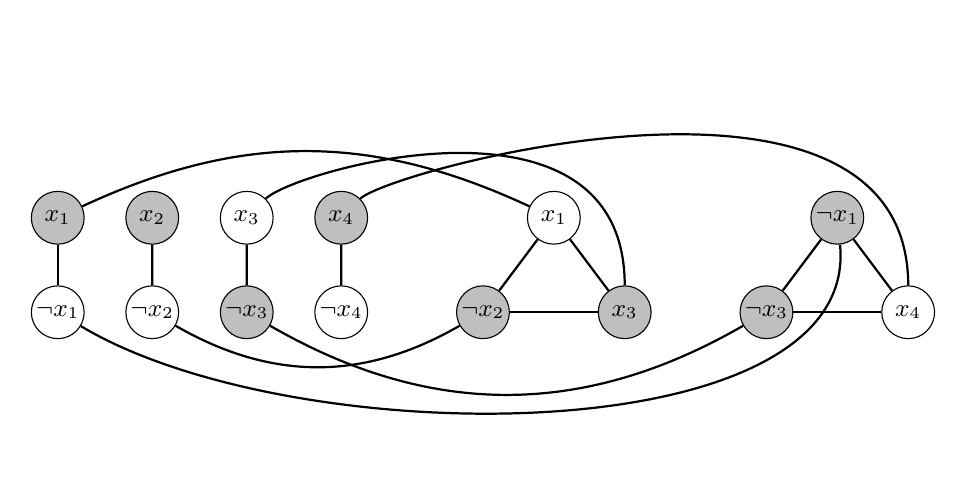
\begin{tikzpicture}[scale=0.6]
\small
\node[draw, circle,fill=lightgray] (a1) at (0,0) {$x_1$};
\node[draw, circle,fill=lightgray] (a2) at (2,0) {$x_2$};
\node[draw, circle] (a3) at (4,0) {$x_3$};
\node[draw, circle,fill=lightgray] (a4) at (6,0) {$x_4$};
\node[draw, circle] (b1) at (0,-2) {\phantom{$x_1$}};
\node[draw, circle] (b2) at (2,-2) {\phantom{$x_2$}};
\node[draw, circle,fill=lightgray] (b3) at (4,-2) {\phantom{$x_3$}};
\node[draw, circle] (b4) at (6,-2) {\phantom{$x_4$}};
\node at (0,-2) {$\neg x_1$};
\node at (2,-2) {$\neg x_2$};
\node at (4,-2) {$\neg x_3$};
\node at (6,-2) {$\neg x_4$};

\node[draw, circle] (c1) at (10.5,0) {$x_1$};
\node[draw, circle,fill=lightgray] (c2) at (9,-2) {\phantom{$x_2$}};
\node[draw, circle,fill=lightgray] (c3) at (12,-2) {$x_3$};
\node at (9,-2) {$\neg x_2$};

\node[draw, circle,fill=lightgray] (d1) at (16.5,0) {\phantom{$x_1$}};
\node[draw, circle,fill=lightgray] (d2) at (15,-2) {\phantom{$x_3$}};
\node[draw, circle] (d3) at (18,-2) {$x_4$};
\node at (16.5,0) {$\neg x_1$};
\node at (15,-2) {$\neg x_3$};

\path[draw,thick,-] (a1) -- (b1);
\path[draw,thick,-] (a2) -- (b2);
\path[draw,thick,-] (a3) -- (b3);
\path[draw,thick,-] (a4) -- (b4);

\path[draw,thick,-] (c1) -- (c2);
\path[draw,thick,-] (c2) -- (c3);
\path[draw,thick,-] (c3) -- (c1);
\path[draw,thick,-] (d1) -- (d2);
\path[draw,thick,-] (d2) -- (d3);
\path[draw,thick,-] (d3) -- (d1);

\path[draw,thick,-] (a1) edge [bend left=25] (c1);
\path[draw,thick,-] (b2) edge [bend right=30] (c2);
\path[draw,thick,-] (b3) edge [bend right=30] (d2);

\path[draw,thick,-] (a3) .. controls (5,1) and (12,3.00) .. (c3);
\path[draw,thick,-] (a4) .. controls (7,1) and (18,4.00) .. (d3);
\path[draw,thick,-] (b1) .. controls (5,-5) and (17,-5.00) .. (d1);
\end{tikzpicture}
\end{center}
\caption{Ratkaisu, jossa $x_1$, $x_2$ ja $x_4$ ovat tosia ja $x_3$ on epätosi.}
\label{fig:solko2}
\end{figure}

Osoittautuu, että voimme saada kaavan todeksi tarkalleen silloin,
kun verkossa on solmupeite, jossa on enintään $n+2m$ solmua.
Tällaiseen peitteeseen kuuluu toinen solmu jokaisesta
parista $x_i$ ja $\neg x_i$, mikä määrittää, miten muuttujien
arvot asetetaan.
Lisäksi peitteeseen kuuluu kaksi solmua jokaisesta kolmen solmun ryhmästä.
Koska ryhmässä on yksi solmu, joka ei kuulu peitteeseen,
sen täytyy olla yhteydessä kaarella solmuun, joka kuuluu peitteeseen.
Tämä varmistaa, että jokaisessa lausekkeessa ainakin yksi kolmesta
muuttujasta on asetettu oikein.

Olemme siis onnistuneet palauttamaan 3SAT-ongelman solmupeiteongelmaksi
niin, että verkon koko on polynominen suhteessa kaavan pituuteen,
joten solmupeiteongelma on NP-täydellinen.

\subsection{Lisää ongelmia}

Palautusten avulla on onnistuttu löytämään tuhansia NP-täydellisiä ongelmia.
Esimerkiksi myös seuraavat ongelmat ovat NP-täydellisiä:

\begin{itemize}
\item onko verkossa $k$-kokoista \emph{klikkiä} eli $k$ solmun joukkoa,
jossa jokaisen kahden solmun välillä on kaari?
\item voimmeko värittää verkon solmut kolmella värillä niin,
että jokaisen kaaren päätesolmut ovat erivärisiä?
\item onko verkossa polkua, joka kulkee tasan kerran jokaisen
verkon solmun kautta (eli \emph{Hamiltonin polkua})?
\item voiko annetuista $n$ luvusta valita osajoukon, jonka summa on $x$?
\end{itemize}

Entä millainen olisi ongelma, jonka ei tiedetä kuuluvan luokkaan P
eikä olevan NP-täydellinen?
Klassinen esimerkki on ongelma, jossa haluamme tutkia,
ovatko kaksi verkkoa \emph{isomorfiset} eli onko niiden
rakenne samanlainen.
Tähän ongelmaan ei tunneta polynomiaikaista algoritmia,
mutta ei ole myöskään tiedossa tapaa palauttaa
jotain NP-täydellistä ongelmaa siihen.

\subsection{Optimointiongelmat}

Käytännössä haluamme usein ratkaista päätösongelman
sijasta \emph{optimointiongelman}: haluamme etsiä pienimmän
tai suurimman mahdollisen ratkaisun.
Esimerkiksi emme halua tarkastaa, onko verkossa
enintään $k$ solmun solmupeitettä (päätösongelma),
vaan haluamme etsiä \emph{pienimmän} solmupeitteen (optimointiongelma).
Osoittautuu kuitenkin, että päätösongelmat ja optimointiongelmat
ovat loppujen lopuksi hyvin lähellä toisiaan.

Oletetaan, että meillä on keino tarkastaa tehokkaasti,
onko verkossa enin\-tään $k$ solmun solmupeitettä.
Miten voimme menetellä, jos haluammekin etsiä pienimmän
solmupeitteen?
Ratkaisuna on käyttää \emph{binäärihakua}:
etsimme pienimmän arvon $x$, jolle pätee,
että verkossa on enintään $x$ solmun solmupeite.
Tämä tarkoittaa, että verkon pienin solmupeite
sisältää $x$ solmua.
Koska käytämme binäärihakua, meidän riittää ratkaista
päätösongelma logaritminen määrä kertoja,
joten saamme ratkaistua optimointiongelman lähes yhtä
tehokkaasti kuin päätösongelman.

Sanomme, että ongelma on \emph{NP-vaikea}, jos voimme palauttaa
kaikki luokan NP ongelmat siihen mutta ongelman ei
tarvitse itse kuulua luokkaan NP.
Jos ongelma on NP-vaikea, se on siis ainakin yhtä vaikea
kuin luokan NP vaikeimmat ongelmat.
Tyypillisiä NP-vaikeita ongelmia ovat NP-täydellisten
päätösongelmien optimointiversiot,
koska voimme palauttaa niihin NP-täydellisiä ongelmia
mutta ne eivät itse kuulu luokkaan NP.

Käytännössä termejä ei käytetä aina näin täsmällisesti
ja optimointiongelmaa saatetaan sanoa NP-täydelliseksi,
vaikka se oikeastaan on NP-vaikea.
Voimme myös vain puhua yleisesti NP-ongelmista,
kun tarkoitamme NP-täydellisiä tai NP-vaikeita ongelmia.

\section{Ongelmien ratkaiseminen}

Jos saamme ratkaistavaksemme NP-ongelman,
tilanne ei näytä hy\-vältä, koska edessämme on silloin ongelma,
johon ei tunneta mitään tehokasta algoritmia.
Emme voi toivoa, että osaisimme ratkaista tehokkaasti ongelmaa,
jota kukaan muukaan ei ole osannut,
etenkin kun yleisesti uskotaan, että $\textrm{P} \neq \textrm{NP}$.
Peli ei ole kuitenkaan välttämättä menetetty.

Suoraviivainen tapa koettaa ratkaista NP-ongelmaa on 
käyttää peruuttavaa hakua, joka käy läpi kaikki mahdolliset
ratkaisut raa'alla voimalla.
Tässä tulee kuitenkin ongelmaksi haun hitaus,
eikä haku löydä välttämättä mitään järkevää ratkaisua alkuvaiheessa.
Käytännössä voimme usein tyytyä siihen,
että löydämme nopeasti \emph{melko hyvän} ratkaisun,
vaikka se ei olisi optimaalinen.
Voimme koettaa muodostaa ratkaisun ahneesti niin,
että käytämme sopivaa \emph{heuristiikkaa},
joka ohjaa hakua hyvältä näyttävään suuntaan.
Voimme myös hyödyntää \emph{satunnaisuutta} niin,
että algoritmi arpoo suuren määrän ratkaisuja
ja valitsee niistä parhaan.
Näiden ainesten avulla on saatu aikaan käytännössä
hyviä ratkaisuja monissa vaikeissa ongelmissa.

Esimerkiksi jos haluamme löytää verkosta suuren klikin,
voimme järjestää verkon solmut satunnaiseen järjestykseen
ja muodostaa klikin käymällä solmut läpi ja lisäämällä
solmun klikkiin, jos siitä on kaari kaikissa klikissä
tällä hetkellä oleviin solmuihin.
Kun toistamme tätä monta kertaa, löydämme todennäköisesti
jonkin klikin, joka on lähellä verkon suurinta klikkiä.
Toisaalta emme voi tietää koskaan varmasti,
onko suurin löytynyt klikki suurin mahdollinen,
koska käymme läpi vain satunnaisia järjestyksiä emmekä
kaikkia mahdollisia vaihtoehtoja, mikä olisi liian hidasta.

Joskus voimme saada aikaan NP-ongelmaan \emph{pseudopolynomisen}
ratkaisun dynaamisen ohjelmoinnin avulla.
Tämä tarkoittaa, että algoritmi näyttää päältä päin polynomiselta,
mutta sen tehokkuus perustuu siihen,
että teemme oletuksia syötteen lukujen suuruudesta.
Tyypillinen esimerkki on NP-täydellinen ongelma,
jossa haluamme muodostaa $n$ kokonaisluvusta osajoukon,
jonka summa on $x$.
Voimme ratkaista tehtävän dynaamisella ohjelmoinnilla niin,
että ratkaisun aikavaativuus on $O(ns)$, missä $s$
on lukujen summa.
Tällainen ratkaisu on tehokas monissa käytännön tilanteissa,
kunhan $s$ on riittävän pieni.
Kuitenkin yleisessä tilanteessa luvut voivat olla
suuria emmekä voi enää käyttää dynaamista ohjelmointia.